\chapter{Background theory}\label{Background_theory}

\section{ADC Converters Fundamentals }\label{fundamentals}

The structure of an typical ADC is shown in the figure \ref{fig:adc_block}. It consists of four main blocks: an anti aliasing filter(AAF), a sample and hold circuit(S/H), a quantizer and a digital filter(decimator).
\begin{figure}[h]
\centering
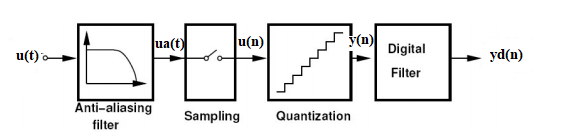
\includegraphics[scale=0.9]{images/adc_block.png}
\caption{Block diagram of a an ADC}
\label{fig:adc_block}
\end{figure}

The AAF is placed in front of the S/H circuit to remove spectral components higher than the bandwidth $\mid\frac{f_s}{2}\mid$ from the input signal $u(t)$, where $f_s$ is the sampling frequency. Thus by band-limiting the signal, it makes sure that the S/H circuit won't fold unwanted high spectral components into the band of interest. Despite being an essential block of the converters, its function is not considered as part of the conversion process.

After the signal has been conditioned to a band, the AAF's output $u_a(t)$ is sampled by the S/H circuit at the sampling frequency $f_s$. The output of the circuit will be $u(n) = u_a(nT_s)$, where $T_s$ is the sampling period($\frac{1}{f_s}$), and n is an integer in the range of 0 and the total number of samples. The next stage of the conversion process is done by the quantizer. It takes a continuous values of the sample data $u(n)$, and maps them onto a finite number of discrete values/levels. Since the quantizer is not ideal, it will introduce a distinction between the mapped values and the actual analog value. This distinction is often called the quantization error($\epsilon_Q$) that is often referred to as the quantization noise of the ADC. If we assume that the quantizer's input signal $u(n)$ varies quite rapidly, then we approximate the quantizer noise to a uniformly distributed additive white noise. Hence we usually choose to model the quantizer noise as white noise with the average power given by the following expression: 

\begin{equation}
    P_E = \frac{\Delta^2}{12},
\end{equation}

where 

\begin{equation}
    \Delta = \frac{V_{FS}}{k},
\end{equation}

$V_{FS}$ is the full-scale of the quantizer, while $k$ is the number levels the quantizer consists of. Meaning if we have a N-bit quantizer, then the number of levels is given by $k = 2^N - 1$. 

The output signal $y(n)$ of the quantizer is a digital pulse train that gets sent to the digital filter. The digital filter performs low-pass filtering and down-sampling on the signal $y(n)$ to eliminate out of band noise above the bandwidth $\frac{f_s}{2}$, and providing an output with Nyquist rate with bit width corresponding to the ADC's resolution. 

\section{Performance Metrics}

There are many metrics used to determine the performance of an ADC as shown in \cite{Allen}, \cite{Johns}, \cite{Razavi}, \cite{Barker}, \cite{Malo} and \cite{Plass}. We will look at those which are most useful to measure the performance of a $\Delta\Sigma$ modulator. These are used to analyze the output spectrum of the modulator. For example we can obtain metrics such as SNR, SNDR, DR and ENOB by analyzing outputs as depicted in figure \ref{fig:metrics} for a determined input power. 

\subsection{Resolution}
Resolution of a converter is defined as the distinct number of analog levels corresponding to the different digital words. Thus, if the ADC has a N-bit resolution, the converter can resolve $2^N$ distinct analog levels.

\subsection{Dynamic Range (DR)}
Dynamic range of an ADC is defined as the range of amplitudes the ADC can effectively resolve. The ADC can overload if the signal is too large, and can get lost in the quantization noise if it too small. It can be defined in two ways. One being the ratio of the full scale value to the smallest difference it can resolve i.e. $V_{LSB}$

\begin{equation}
    DR = 6.02N.
\end{equation}

The other definition being the power of the input signal where the SNR (or the SNDR) is $0dB$. 

\subsection{Signal-to-Noise ratio (SNR)}
Signal-to-noise ratio is the ratio between the signal power and the total noise power at the output. When the case is only quantization noise, it is called signal-to-quantization-noise ratio(SQNR). 

\subsection{Signal-to-noise-distortion ratio (SNDR)}
SNDR is the ratio of the signal power to the total noise and the harmonic power at the output. The parameter is also called signal-to-noise and distortion ratio(SINAD).  

\subsection{Spurious Free Dynamic Range (SFDR)}
SFDR is defined as the ratio between the RMS value of the input sine wave for an ADC and the RMS value of the peak spur(the strongest harmonic component power) observed in the frequency domain. Some communication application require maximizing the dynamic range of the converter, here SFDR is an important parameter. 

\subsection{Total Harmonic Distortion (THD)}
THD is defined  as the ratio between the sum of the powers of the harmonic frequencies inside the signal bandwidth and the power of the fundamental frequency. Thus the definition can be expressed as:
\begin{equation}
    THD = \frac{\sum Harmonic frequencies}{Fundamental frequency} = \sqrt{\frac{V_2^2 + V_3^2 + .. +}{V_1^2}}
\end{equation}

\subsection{Effective Number of Bits (ENOB)}
This metric gives actual number of bits for a given SNDR or SINAD. It is defined by the following equation:

\begin{equation}
    ENOB = \frac{SNR - 1.76}{6.02}
\end{equation}

\subsection{Overload level}
It is the maximum level of input amplitude for which the system can still operate correctly. 
\begin{figure}[ht]
\centering
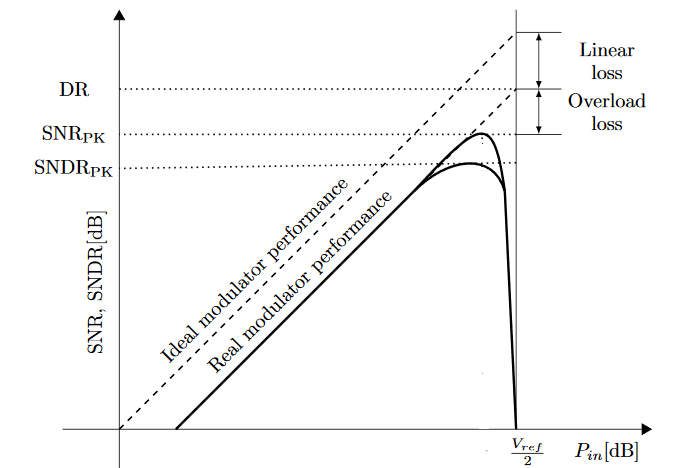
\includegraphics[scale=0.5]{images/metrics_snr.png}
\caption{Typical SNR vs. Input power}
\label{fig:metrics}
\end{figure}

\section{Classification of Data Converters}
Which category the data converters is placed in is influenced by the sampling frequency used for the conversion process. Broadly speaking the data converters can be classified into two categories; Nyquist-rate -and oversampling converters\cite{Ovi}.  

\subsection{Nyquist-Rate Converters}
The Nyquist-rate converters are based on the well known sampling theorem also known as the Nyquist theorem, which state the sampling frequency $f_2$ should be at least twice as large as the bandwidth $f_b$ in order to avoid aliasing and successfully reproduce the signal after filtering. Hence it will use an input occupying a large portion of the available bandwidth. The quantization noise in a Nyquist-rate converter is given by expression: 2.1. In Nyquist-rate converters, the sampling frequency is usually at least twice the signal bandwidth. The maximum SQNR of a Nyquist-rate converter can be obtained\cite{Richard}[Chapter 1.1], as seen in expression(2.4), where N is the number of bits.

\begin{equation}\label{no_noise_sqnr}
    SQNR_{maxNQ} = 6.02N + 1.76 dB
\end{equation}

\subsection{Oversampling Converters}
In the preceding section it was mentioned that Nyquist-rate converters will use an input occupying a large potion of the available bandwidth. Oversampling converters on the other hand only occupy a small portion of the bandwidth, thus spreading the quantization noise over a wider frequency range as depicted in figure \ref{fig:oversample}. This causes the quantization noise to be reduced.  

\begin{figure}[h]
\centering
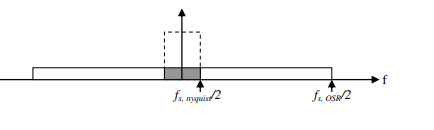
\includegraphics[scale=1]{images/oversample.png}
\caption{Quantization noise spectrum of a Nyquist-rate and a oversampling converter}
\label{fig:oversample}
\end{figure}

To be able to operate in such small portion of the bandwidth, the oversampling converters have to sample the input signal in a much higher rate than the Nyquist-rate converters. This rate is given by the oversampling ratio (OSR) which is defined as,

\begin{equation}
    OSR = \frac{f_s}{2f_b}
\end{equation}

To establish the advantage of oversampling converters compared to Nyquist-rate converters, we can look at the maximum signal-to-quantization-noise ratio (SQNR) for a oversampling converter. It can be calculated for oversampling converters\cite{Johns}[Ch 18.3], as seen in expression (2.8), where N is the number of bits.


\begin{equation}
    SQNR_{maxOS} = 6.02N + 1.76 + 10\log_{10}(OSR) dB
\end{equation}

If we compare equation (2.8) with equation (2.6), we can see that the oversampling rate ADC can achieve the same SQNR performance as a Nyquist-rate ADC with fewer bits. Further it can be seen that for every doubling of OSR improves the SQNR with $3 dB$, or effective number of bits (ENOB) by $0.5bits/octave$. 

Another advantage of using oversampling ADCs is that the specifications of the AAF are relaxed, because the signal bandwidth is smaller than $\frac{f_s}{2}$. As shown in figure \ref{fig:AAF}, the spectral components higher than the bandwidth $f_b$ in a oversampling converter are more separated than in a Nyquist-rate converter. 

\begin{figure}
\centering
\begin{subfigure}[b]{0.35\textwidth}
   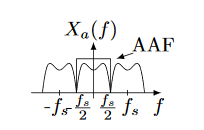
\includegraphics[width=1\linewidth]{images/nyquist_aaf.png}
   \caption{Anti aliasing filter for Nyquist-rate converter}
   \label{fig:AAf_NQ} 
\end{subfigure}

\begin{subfigure}[b]{0.55\textwidth}
   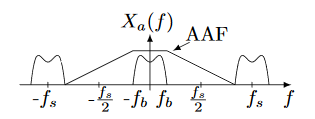
\includegraphics[width=1\linewidth]{images/over_aaf.png}
   \caption{Anti aliasing filter for Oversampling converter}
   \label{fig:AAF_OV}
\end{subfigure}

\caption{Anti aliasing filter for Nyquist-rate and Oversampling converters}
\label{fig:AAF}
\end{figure}

\section{Noise-Shaping ADC}
To get a better understanding of noise-shaping, we have to first look at the $\Delta\Sigma$ modulator. The structure of typical $\Delta\Sigma$ ADC is shown in figure \ref{fig:delta_block}, which consists of four main blocks: a AAF, a S/H circuit, a $\Delta\Sigma$ modulator and a decimator. The AAF, S/H circuit and the decimator operates as explained in section \ref{fundamentals}.

\begin{figure}[h]
\centering
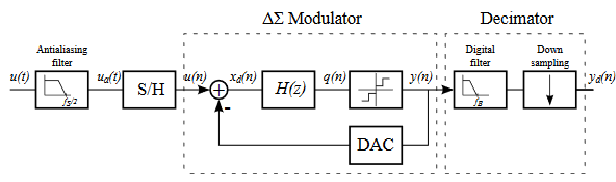
\includegraphics[scale=0.8]{images/delta_sigma_block.png}
\caption{Block diagram of a discrete-time (DT) $\Delta\Sigma$ ADC\cite{deltapic}}
\label{fig:delta_block}
\end{figure}

Even though all four blocks are essential to the ADC, our main focus for this thesis is the $\Delta\Sigma$ modulator. As shown from the figure \ref{fig:delta_block}, the $\Delta\Sigma$ modulator consists of a loop filter ($H(z)$) along with an internal quantizer and a DAC, which together makes a negative feedback loop. The basic operation of the modulator is to compare the input signal with an estimate of the output data and quantizing this error. This structure is advantageous for oversampling signals since the amplitude of the subtracted signal $x_d(n)$ is smaller than for the input signal $u(n)$. By having a loop filter with a very high gain in the signal band, the in-band quantization noise is strongly attenuated by the feedback loop. The input signal will nearly pass unaffected through to the output. This process is known as \textit{noise-shaping}.

\section{First Order $\Delta\Sigma$ Modulator}\label{first_order}
To get the basic understanding in how this system works, a linear model of the $\Delta\Sigma$ modulator is shown in figure \ref{fig:linear}. The quantizer is replaced with its noise source \textit{e(n)} which we assume is white noise, and the DAC is replaced with a wire since we assume it is ideal. The system can be described by the transfer from each of the independent inputs: \textit{e(n)} and \textit{u(n)} to the output \textit{y(n)}. 

\begin{equation}
    Y(Z) = \frac{H(z)}{1+H(z)}U(z) + \frac{1}{1+H(z)}E(z)
\end{equation}

Here we can define signal transfer function \textit{STF} and noise transfer function \textit{NTF} as

\begin{equation}\label{stf_1}
    STF(z) = \frac{H(z)}{1+H(z)}U(z)
\end{equation}

and

\begin{equation}\label{ntf_1}
    NTF(z) = \frac{1}{1+H(z)}E(z)
\end{equation}

As mentioned the loop filter \textit{H(z)} has to have high gain in-band, while it may decrease outside. A commonly used filter is the delaying discrete time integrator

\begin{equation}\label{Hz}
    H(z) = \frac{z^{-1}}{1-z^{-1}}
\end{equation}

By inserting equation \ref{Hz} onto \ref{stf_1} and \ref{ntf_1}, we get

\begin{equation}\label{stf_2}
    STF(z) = \frac{\frac{z^{-1}}{1-z^{-1}}}{1 + \frac{z^{-1}}{1-z^{-1}}} = z^{-1}
\end{equation}

and

\begin{equation}\label{ntf_2}
    NTF(z) = \frac{1}{1 + \frac{z^{-1}}{1 - z^{-1}}} = 1 - z^{-1}
\end{equation}

\begin{figure}[h]
\centering
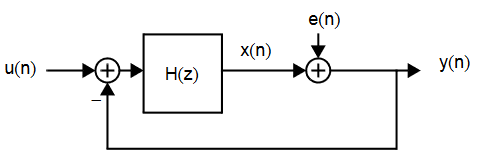
\includegraphics[scale=0.8]{images/linear_delta.png}
\caption{Linear model of $\Delta\Sigma$ modulator with inclusion of quantization noise \cite{Johns}}
\label{fig:linear}
\end{figure}

We can see from equation \ref{ntf_2} that the NTF is a high-pass filter. Therefore the in-band noise that resides on the lower frequency will be attenuated, and we can see the \textit{noise-shaping} feature of the $\Delta\Sigma$ modulator. The STF \ref{stf_2} becomes a simple unit delay. This is seen as first order $\Delta\Sigma$ modulator, and the maximum SQNR is given in \cite[Ch.18.2.2]{Johns}

\begin{equation}\label{SQNR_noise}
  SQNR_{max} = 6.02N + 1.76 - 5.17 + 30log_{10}(OSR)  
\end{equation}

From equation \ref{SQNR_noise}, it can be noticed that for every doubling of OSR, the SQNR improves with 9dB or, ENOB with 1.5bits/octave. Compared with oversampling with no noise shaping expression \ref{no_noise_sqnr}, we can see that the improvement is three times as good. 

In the next chapter while exploring the different aspects of the $\Delta\Sigma$ modulator, we will see how increasing the order of the loop filter H(z), can further improve the noise-shaping and thereby improve the $SQNR_{max}$. 